First of all, the shape of the simulated tritated water source was optimized. The mean free path of tritium electrons in water is only around $5~\mu\meter$, so most electrons do not reach the scintillating fibers. These electrons do not provide useful information and only consume computing resources. To optimize the simulation, the dimensions of the simulated tritium source were tested to minimizes the number of tritium events that do not reach the scintillating fibers. 

Before that, the initial energy distribution of the simulated tritium events was checked, shown in figure \ref{subfig:EnergyDistributionTritiumSource}, and compared with the input taken from \cite{TritiumEmissionSpectrum}, obtaining a good agreement between both. In addition, the distribution of the initial energy of tritium electrons capable of penetrating a fiber and depositing energy is compared to the initial energy distribution of all simulated tritium events, Figure \ref{subfig:EnergySpectrumEventsDetectedandNonDetected}. A shift to high energies is observed, creating a peak centred at $10~\keV$. This shift occurs because the lower energy tritium electrons do not have enough energy to reach and penetrate the fiber and are not detected.

\begin{figure}
\centering
    \begin{subfigure}[b]{0.45\textwidth}
    \centering
    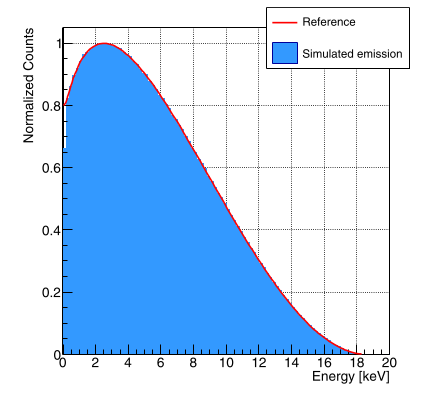
\includegraphics[width=\textwidth]{8SimulationsResults/81TRITIUMDesign/811TritiumSourceOptimization/TritiumSourceEnergyDistribution.png}  
    \caption{\label{subfig:EnergyDistributionTritiumSource}}
    \end{subfigure}
    \hfill
    \begin{subfigure}[b]{0.45\textwidth}
    \centering
    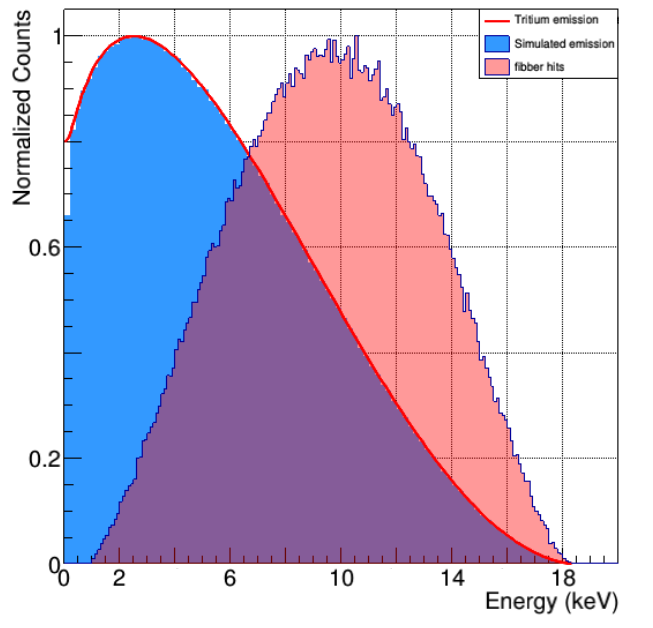
\includegraphics[width=\textwidth]{8SimulationsResults/81TRITIUMDesign/811TritiumSourceOptimization/Source_Spectrum_yes_and_non_detected_events.png}  
    \caption{\label{subfig:EnergySpectrumEventsDetectedandNonDetected}}
    \end{subfigure}
 \caption{Energy distribution of a) simulated tritium decays b) Initial energy of tritium decays that reach the scintillating fibers (red histogram) compared the all simulated tritium events (blue histogram) \cite{SimulationPaperCarlos}.
 \label{fig:TritiumSourceOptimization}}
\end{figure}

Regarding the optimization of the tritium source shape, a scintillating fiber $20~\cm$ long and $2~\mm$ in diameter and a surrounding tritiated water source of the same length and $0.5~\mm$ thick, $100$ times greater that the mean free path of tritium electrons, were simulated to assess the tritium source. The dimensions of the fiber are not important in this study since only the energy deposition of tritium electrons in the fiber were simulated, excluding optical processes. The objective of this simulation is to find the radial thick of the simulated tritium source at which non significant amount of tritium decay electrons are generated. In Figure \ref{subfig:TransversalCutTritiumSource}, a transversal cut of the $2~\mm$ scintillating fiber, the simulated tritium source $0.5~\mm$ thick around the fiber, and the position where the tritium decays happen, the electrons of which has deposited their energy in the scintillating fiber are shown. Furthermore, the distribution of the radial distance between the position where tritium decays take place and the surface of the scintillating fiber is shown in figure \ref{subfig:DistanceDistributionTritiumSourceFiber}. As can be seen in the Figure \ref{fig:TritiumSourceSimulated}, most of the tritium decays that are detected occur in close proximity to the scintillating fiber.  A zoom is applied in the inset box of the Figure \ref{subfig:DistanceDistributionTritiumSourceFiber} for better viewing. The chosen thickness of the simulated tritium source is $5~\mu\meter$ since the $99.4\%$ of the events that are able to deposit energy in fibers are produced at most at this distance.

\begin{figure}
\centering
    \begin{subfigure}[b]{0.45\textwidth}
    \centering
    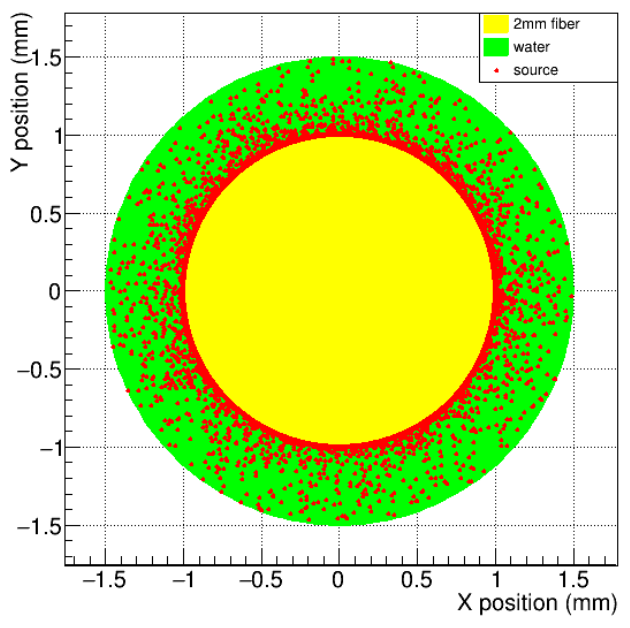
\includegraphics[width=\textwidth]{8SimulationsResults/81TRITIUMDesign/811TritiumSourceOptimization/Source_Ring.png}  
    \caption{\label{subfig:TransversalCutTritiumSource}}
    \end{subfigure}
    \hfill
    \begin{subfigure}[b]{0.45\textwidth}
    \centering
    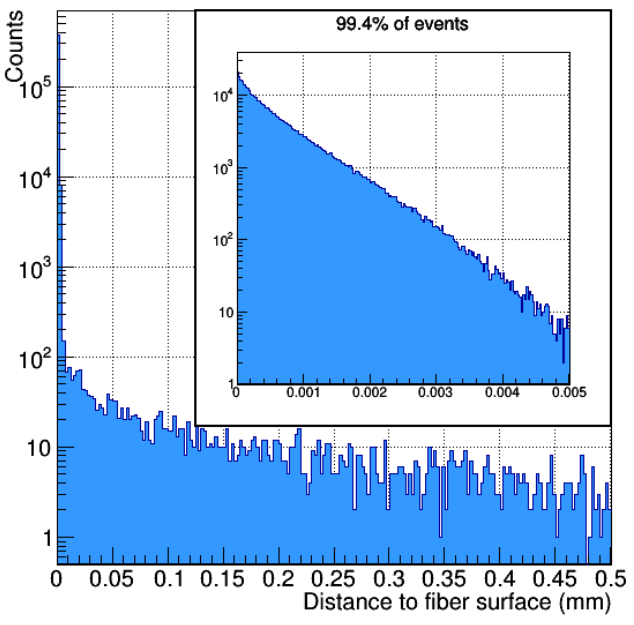
\includegraphics[width=\textwidth]{8SimulationsResults/81TRITIUMDesign/811TritiumSourceOptimization/SourceDistance.png}  
    \caption{\label{subfig:DistanceDistributionTritiumSourceFiber}}
    \end{subfigure}
 \caption{a)Transversal cut of simulated scintillating fiber (yellow) and tritium source (green) with various tritium decays (red dots) b) Distribution of the radial distance between the position where the tritium decay takes place and the surface of the scintillating fiber \cite{SimulationPaperCarlos}.}
 \label{fig:TritiumSourceSimulated}
\end{figure}	

